%%%%%%%%%%%%%%%%%%%%%%%%%%%%%%%%%%%%%%%%%%%%%%%%%%%%%%%%%%%%%%%%
%
%  Template for homework of Introduction to Machine Learning.
%
%  Fill in your name, lecture number, lecture date and body
%  of homework as indicated below.
%
%%%%%%%%%%%%%%%%%%%%%%%%%%%%%%%%%%%%%%%%%%%%%%%%%%%%%%%%%%%%%%%%


\documentclass[11pt,letter,notitlepage]{article}
%Mise en page
\usepackage[left=2cm, right=2cm, lines=45, top=0.8in, bottom=0.7in]{geometry}
\usepackage{fancyhdr}
\usepackage{fancybox}
\usepackage{graphicx}
\usepackage{pdfpages}
\usepackage[UTF8]{ctex}
\usepackage{enumitem}
\usepackage{algorithm}
\usepackage{algorithmic}
\renewcommand{\headrulewidth}{1.5pt}
\renewcommand{\footrulewidth}{1.5pt}
\newcommand\Loadedframemethod{TikZ}
\usepackage[framemethod=\Loadedframemethod]{mdframed}

\usepackage{amssymb,amsmath}
\usepackage{amsthm}
\usepackage{thmtools}
\newtheorem{lemma}{Lemma}

\setlength{\topmargin}{0pt}
\setlength{\textheight}{9in}
\setlength{\headheight}{0pt}

\setlength{\oddsidemargin}{0.25in}
\setlength{\textwidth}{6in}

\usepackage{graphicx} % more modern
\usepackage{subfigure}

%%%%%%%%%%%%%%%%%%%%%%%%
%%%%%% Define math operator %%%%%
%%%%%%%%%%%%%%%%%%%%%%%%
\DeclareMathOperator*{\argmin}{\bf argmin}
\DeclareMathOperator*{\relint}{\bf relint\,}
\DeclareMathOperator*{\dom}{\bf dom\,}
\DeclareMathOperator*{\intp}{\bf int\,}
%%%%%%%%%%%%%%%%%%%%%%%


\setlength{\topmargin}{0pt}
\setlength{\textheight}{9in}
\setlength{\headheight}{0pt}

\setlength{\oddsidemargin}{0.25in}
\setlength{\textwidth}{6in}
\pagestyle{fancy}
%%%%%%%%%%%%%%%%%%%%%%%%
%% Define the Exercise environment %%
%%%%%%%%%%%%%%%%%%%%%%%%
\mdtheorem[
topline=false,
rightline=false,
leftline=false,
bottomline=false,
leftmargin=-10,
rightmargin=-10
]{exercise}{\textbf{Exercise}}
%%%%%%%%%%%%%%%%%%%%%%%
%% End of the Exercise environment %%
%%%%%%%%%%%%%%%%%%%%%%%


%%%%%%%%%%%%%%%%%%%%%%%%
%% Define the Problem environment %%
%%%%%%%%%%%%%%%%%%%%%%%%
\mdtheorem[
topline=false,
rightline=false,
leftline=false,
bottomline=false,
leftmargin=-10,
rightmargin=-10
]{problem}{\textbf{Problem}}
%%%%%%%%%%%%%%%%%%%%%%%
%% End of the Exercise environment %%
%%%%%%%%%%%%%%%%%%%%%%%

%%%%%%%%%%%%%%%%%%%%%%%
%% Define the Solution Environment %%
%%%%%%%%%%%%%%%%%%%%%%%
\declaretheoremstyle
[
spaceabove=0pt, 
spacebelow=0pt, 
headfont=\normalfont\bfseries,
notefont=\mdseries, 
notebraces={(}{)}, 
headpunct={:\quad}, 
headindent={},
postheadspace={ }, 
postheadspace=4pt, 
bodyfont=\normalfont, 
qed=$\blacksquare$,
preheadhook={\begin{mdframed}[style=myframedstyle]},
	postfoothook=\end{mdframed},
]{mystyle}

\declaretheorem[style=mystyle,title=Solution,numbered=no]{solution}
\mdfdefinestyle{myframedstyle}{%
	topline=false,
	rightline=false,
	leftline=false,
	bottomline=false,
	skipabove=-6ex,
	leftmargin=-10,
	rightmargin=-10}
%%%%%%%%%%%%%%%%%%%%%%%
%% End of the Solution environment %%
%%%%%%%%%%%%%%%%%%%%%%%

%% Homework info.
\newcommand{\posted}{\text{Nov. 5, 2019}}       			%%% FILL IN POST DATE HERE
\newcommand{\due}{\text{Nov. 18, 2019}} 			%%% FILL IN Due DATE HERE
\newcommand{\hwno}{\text{4}} 		           			%%% FILL IN LECTURE NUMBER HERE


%%%%%%%%%%%%%%%%%%%%
%% Put your information here %%
%%%%%%%%%%%%%%%%%%%
\newcommand{\name}{\text{Bowen Zhang}}  	          			%%% FILL IN YOUR NAME HERE
\newcommand{\id}{\text{PB17000215}}		       			%%% FILL IN YOUR ID HERE
%%%%%%%%%%%%%%%%%%%%
%% End of the student's info %%
%%%%%%%%%%%%%%%%%%%


\newcommand{\proj}[2]{\textbf{P}_{#2} (#1)}
\newcommand{\lspan}[1]{\textbf{span}  (#1)  }
\newcommand{\rank}[1]{ \textbf{rank}  (#1)  }
\newcommand{\RNum}[1]{\uppercase\expandafter{\romannumeral #1\relax}}


\lhead{
	\textbf{\name}
}
\rhead{
	\textbf{\id}
}
\chead{\textbf{
		Homework \hwno
}}


\begin{document}
\vspace*{-4\baselineskip}
\thispagestyle{empty}


\begin{center}
{\bf\large Introduction to Machine Learning}\\
{Fall 2019}\\
University of Science and Technology of China
\end{center}

\noindent
Lecturer: Jie Wang  			 %%% FILL IN LECTURER HERE
\hfill
Homework \hwno             			
\\
Posted: \posted
\hfill
Due: \due
\\
Name: \name             			
\hfill
ID: \id						
\hfill

\noindent
\rule{\textwidth}{2pt}

\medskip





%%%%%%%%%%%%%%%%%%%%%%%%%%%%%%%%%%%%%%%%%%%%%%%%%%%%%%%%%%%%%%%%
%% BODY OF HOMEWORK GOES HERE
%%%%%%%%%%%%%%%%%%%%%%%%%%%%%%%%%%%%%%%%%%%%%%%%%%%%%%%%%%%%%%%%

\textbf{Notice, }to get the full credits, please show your solutions step by step.

\begin{exercise}[Support Vector Machine (SVM) for Linearly Separable Cases \textnormal{40pts}]
Given the training sample $\mathcal{D}=\{ (\textbf{x}_i,y_i) \}_{i=1}^n$, where $\textbf{x}_i \in \mathbb{R}^d$ and $y_i \in \{ -1,1 \}$. Let 
\begin{align*}
    \mathcal{D}^+=\{(\textbf{x}_i,y_i)\in\mathcal{D}:y_i=1\},\hspace{5mm}\mathcal{D}^-=\{(\textbf{x}_i,y_i)\in\mathcal{D}:y_i=-1\}.
\end{align*}
Assume that $\mathcal{D}^+$ and $\mathcal{D}^-$ are nonempty and the training sample $\mathcal{D}$ is linearly separable. We have shown in class that SVM can be written as
\begin{align}\label{prob:SVM-1}
	&\min_{\textbf{w},b}\,\,\frac{1}{2}\| \textbf{w} \|^2, \\
	&\text{ s.t. } \min_i y_{i} ( \langle \textbf{w}, \textbf{x}_i \rangle + b ) = 1. \nonumber
\end{align}
Moreover, we further transform the problem in (\ref{prob:SVM-1}) to
\begin{align}\label{prob:SVM}
    	&\min_{\textbf{w},b}\,\,\frac{1}{2}\| \textbf{w} \|^2, \\
    	&\text{ s.t. }\,\, y_{i} ( \langle \textbf{w}, \textbf{x}_i \rangle + b ) \geq 1, i=1,\ldots,n. \nonumber
\end{align}
We denote the feasible set of the problem in (\ref{prob:SVM}) by $$\mathcal{F}=\{(\mathbf{w},b):y_{i} ( \langle \textbf{w}, \textbf{x}_i \rangle + b ) \geq 1, i=1,\ldots,n\}.$$

\begin{enumerate}
    \item Show that $\mathcal{F}$ is nonempty.
    \item Show that the problem in (\ref{prob:SVM}) admits an optimal solution.
    \item Let $(\textbf{w}^*,b^*)$ be the optimal solution to problem (\ref{prob:SVM}). Show that $\mathbf{w}^*\neq0$.
    \item Show that the problems in (\ref{prob:SVM-1}) and (\ref{prob:SVM}) are equivalent, that is, they share the same set of optimal solutions.
    \item Let $(\textbf{w}^*,b^*)$ be the optimal solution to problem (\ref{prob:SVM}). Show there exist at least one positive sample and one negative sample, respectively, such that the equality holds. In other words, there exist $i,j \in \{ 1,2,\dots,n \}$ such that 
    \begin{align*}
        1=y_i = &\langle \textbf{w}^*, \textbf{x}_i \rangle + b^*, \\
        -1=y_j = &\langle \textbf{w}^*, \textbf{x}_j \rangle + b^*.
    \end{align*}
    \item Show that the optimal solution to problem (\ref{prob:SVM}) is unique.
    \item Find the dual problem of (\ref{prob:SVM}) and the corresponding optimal conditions.
\end{enumerate}

\end{exercise}
\begin{solution}
	\heiti
	\begin{enumerate}
		\ \\
		\item
			由样本线性可分可知存在 $w_{0} \in \mathbb{R}^d$ 使得:\\
			$\begin{aligned} {\langle w_{0}, x_{i}\rangle > 0 \quad x_{i} \in D^{+}}  \\ {\langle w_{0}, x_{i}\rangle < 0   \quad x_{i} \in D^{-}} \end{aligned}$\\
			所以存在 $\varepsilon, k > 0$ 使得:
			\begin{align*}
				y_{i} \langle w_{0}, x_{i}\rangle &\geqslant \varepsilon \\  \Rightarrow \quad y_{i}\langle \frac{w_{0}}{\varepsilon}, x_{i}\rangle &\geqslant 1
			\end{align*}
			所以令 $w = \frac{w_{0}}{\varepsilon}, b = 0$ 可知 $\mathcal{F}$ 非空。
		\item 
			目标函数只能在有限区间内取到最小值($\mathbf{w} \rightarrow \infty$ 时,目标函数也趋于无穷),而解集非空,故一定存在满足约束条件的最优解。
		\item
			假如 $\mathbf{w}^* = 0$ ,那么有:
			\begin{align*}
				y_i b \geqslant 1, i = 1,\ldots,n.
			\end{align*}
			对 $ y_i = 1$ 有 $b \geqslant 1$,对 $y_i = -1$ 有 $b \leqslant -1$矛盾,故 $\mathbf{w}^* \neq 0$.
		\item 如果两个问题等价,那么当目标函数取到最小值时,$\exists i$ 使得 $y_{i} ( \langle \textbf{w}, \textbf{x}_i \rangle + b ) = 1$.假设问题不等价,那么设问题 2 的最优解为 $(w^*, b^*)$,满足:
		\begin{align*}
			y_{i} ( \langle \textbf{w}^{*}, \textbf{x}_i \rangle + b^{*} ) \geqslant k > 1, i = 1,\ldots,n
		\end{align*}
		那么有:
		\begin{align*}
			y_{i} ( \langle \frac{\textbf{w}^{*}}{k}, \textbf{x}_i \rangle + \frac{b^*}{k} ) \geqslant 1, i = 1,\ldots,n
		\end{align*}
		此时目标函数的值为 $\frac{1}{2}\|\frac{\mathbf{w}^{*}}{k}\|^{2}$,这与 $w^*$ 是最优解矛盾,即问题 2 取到最优解时两个问题的约束条件相同,故两个问题等价。
		\item 由 4 可知必 $\exists i, y_{i} ( \langle \textbf{w}^{*}, \textbf{x}_i \rangle + b^{*} ) = 1$,不妨设这个样本是负样本(正样本证明过程类似,所以只选负样本证明)。如果对所有的正样本都有:
		\begin{align*}
			\langle \textbf{w}^{*}, \textbf{x}_i \rangle + b^{*}  \geqslant k > 1, \textbf{x}_i \in \mathcal{D}^+
		\end{align*}
		对所有的负样本有:
		\begin{align*}
			\langle \textbf{w}^{*}, \textbf{x}_i \rangle + b^{*}  \leqslant -1, \textbf{x}_i \in \mathcal{D}^-
		\end{align*}
		取 $0 < t < k - 1$,稍作变换得:
		\begin{align*}
			\langle \textbf{w}^{*}, \textbf{x}_i \rangle + b^{*} - t  \geqslant k - t > 1, \textbf{x}_i \in \mathcal{D}^+\\
			\langle \textbf{w}^{*}, \textbf{x}_i \rangle + b^{*} - t  \leqslant -1 - t, \textbf{x}_i \in \mathcal{D}^-
		\end{align*}
		即:
		\begin{align*}
			b_0 &= b^{*} - t\\
			y_{i} ( \langle \textbf{w}^{*}, \textbf{x}_i \rangle + b_0 ) &> 1, i = 1,\ldots,n
		\end{align*}
		那么同 4 可证存在更小的 $w$ 使得目标函数取得最小值,这与 $w^*$ 使得目标函数最小矛盾,故命题成立。
		\item 假设存在 $(w_1^*,b_1^*), (w_2^*, b_2^*)$ 两组不同的最优解。假设 $w_1^* \neq w_2^*$,那么有:
		\begin{align*}
			y_{i} ( \langle \textbf{w}_1^{*}, \textbf{x}_i \rangle + b_1^* ) &\geqslant 1, i = 1,\ldots,n\\
			y_{i} ( \langle \textbf{w}_2^{*}, \textbf{x}_i \rangle + b_2^* ) &\geqslant 1, i = 1,\ldots,n\\
			\Rightarrow y_{i} ( \langle \textbf{w}_1^{*} + \textbf{w}_2^{*}, \textbf{x}_i \rangle + b_1^* + b_2^* ) &\geqslant 2, i = 1,\ldots,n\\
			\Rightarrow y_{i} ( \langle \frac{\textbf{w}_1^{*} + \textbf{w}_2^{*}}{2}, \textbf{x}_i \rangle + \frac{b_1^* + b_2^*}{2} ) &\geqslant 1, i = 1,\ldots,n
		\end{align*}
		而
		\begin{align*}
			\| \frac{\textbf{w}_1^{*} + \textbf{w}_2^{*}}{2} \|^2 \leqslant \frac{\| \textbf{w}_1^*\|^2 + \|\textbf{w}_2^* \|^2}{2} =  \|\textbf{w}_1^* \|^2 = \|\textbf{w}_2^* \|^2
		\end{align*}
		因为假设 $w_1^* \neq w_2^*$,所以上式为严格小于。取 $w = \frac{{w}_1^{*} + {w}_2^{*}}{2}$,这说明 $w_1^*, w_2^*$ 不是让目标函数最小的 $w$,所以与 $(w_1^*,b_1^*), (w_2^*, b_2^*)$ 是两组最优解矛盾,故必有 $w_1^* = w_2^*$ 成立。\\
		若 $b_1^* \neq b_2^*$,不妨设 $b_1^* > b_2^*$,由 5 可知存在 $i \in \{1, 2,\dots, n\}$:
		\begin{align*}
			1=y_i &= \langle \textbf{w}^*, \textbf{x}_i \rangle + b_1^*, y_i \in \mathcal{D}^+\\
			&> \langle \textbf{w}^*, \textbf{x}_i \rangle + b_2^*
		\end{align*}
		这与约束条件矛盾,故必有 $b_1^* = b_2^*$。综上最优解唯一。
		\item 引入拉格朗日乘子对偶问题为:
		\begin{align*}
			{ L ( w , b , \alpha ) = \frac { 1 } { 2 } \| w \| ^ { 2 } + \sum _ { i = 1 } ^ { N } \alpha _ { i } \left[ - y _ { i } \left( \langle w \cdot x _ { i } \rangle + b \right) + 1 \right] } \\ { = \frac { 1 } { 2 } \| w \| ^ { 2 } - \sum _ { i = 1 } ^ { N } \alpha _ { i } y _ { i } \left(\langle w, x_i\rangle + b \right) + \sum _ { i = 1 } ^ { N } \alpha _ { i } }
		\end{align*}
		要求解的最优问题为:
		\begin{align*}
			\max_{\alpha} \min_{w, b} L ( w , b , \alpha )
		\end{align*}
		令 $L(w, b, \alpha)$ 对 $w, b$ 的偏导为 0 得:
		\begin{align*}
			w = \sum\limits_{i=1}^{N}\alpha_iy_ix_i,\\
			0 = \sum\limits_{i=1}^{N}\alpha_iy_i.
		\end{align*} 
		代入得到对偶问题为:
		\begin{align*}
			\min_{\alpha} \frac{1}{2}\sum\limits_{i=1}^{N}\sum\limits_{j=1}^{N}\alpha_i\alpha_jy_iy_j\langle x_i, x_j \rangle - \sum\limits_{i=1}^{N} \alpha_i \\
			s.t. \sum\limits_{i=1}^{N}\alpha_iy_i = 0,\\
			\alpha_i \geqslant 0, i= 1,\ldots,n
		\end{align*}
	\end{enumerate}
\end{solution}

\newpage
\begin{exercise}[Visualization Lemma]
Consider the primal problem as follows.
\begin{align}\label{prob:primal-vec}
\min_{\mathbf{x}}\,&f(\mathbf{x})\\ \nonumber
{\rm s.t.}\,&\mathbf{g}(\mathbf{x})\leq0,\\ \nonumber
&\mathbf{h}(\mathbf{x})=0, \\ \nonumber
&\mathbf{x}\in X,
\end{align}
where $\mathbf{x}\in\mathbb{R}^n$, $f:\mathbb{R}^n\rightarrow\mathbb{R}$, $\mathbf{g}:\mathbb{R}^n\rightarrow\mathbb{R}^m$, $\mathbf{h}:\mathbb{R}^n\rightarrow\mathbb{R}^p$, and $X\subseteq\mathbb{R}^n$. The functions $f$, $\mathbf{g}$, and $\mathbf{h}$ are continuously differentiable. 

The Lagrangian $L:\mathbb{R}^n\times \mathbb{R}^m\times \mathbb{R}^p\rightarrow\mathbb{R}$ associated with the problem in (\ref{prob:primal-vec}) takes the form of
\begin{align}\label{def:Lagrangian}
	L(\mathbf{x},\lambda,\mu)=f(\mathbf{x})+\sum_{i=1}^m\lambda_ig_i(\mathbf{x})+\sum_{i=1}^p\mu_ih_i(\mathbf{x}).
\end{align}

Let
\begin{align}\label{def:image-set}
	\mathbb{R}^{m+p+1}\supseteq S=\{(\mathbf{g}(\mathbf{x}),\mathbf{h}(\mathbf{x}),f(\mathbf{x})):\mathbf{x}\in X\}.
\end{align}

Show that the results as follows (hint: see Fig. \ref{fig:visualization-lemma}).

\begin{lemma}
	\textbf{\textup {Visualization Lemma}}
	\begin{enumerate}
		\item The hyperplane with normal $(\lambda,\mu,1)$ that passes through a vector $(\mathbf{g}(\mathbf{x}),\mathbf{h}(\mathbf{x}),f(\mathbf{x}))$ intercepts the vertical axis $\{(\mathbf{0},z):z\in\mathbb{R}\}$ at the level $L(\mathbf{x},\lambda,\mu)$.
		
		\item Among all hyperplanes with normal $(\lambda,\mu,1)$ that contains in their positive halfspace the set $S$ defined in (\ref{def:image-set}), the highest attained level of interception of the vertical axis is $\inf_{\mathbf{x}\in X}\,L(\mathbf{x},\lambda,\mu)$.
		
		\item $(\lambda^*,\mu^*)$ is a geometric multiplier if and only if $\lambda^*\geq0$ and among all hyperplanes with normal $(\lambda^*,\mu^*,1)$ that contain in their positive halfspace the set $S$, the highest attained level of of interception of the vertical axis is $f^*$, where
		\begin{align*}
		    f^*=\min\{f(\mathbf{x}):\mathbf{g}(\mathbf{x})\leq0,\mathbf{h}(\mathbf{x})=0,\mathbf{x}\in X)\}.
		\end{align*}
	\end{enumerate}
\end{lemma}
\end{exercise}
\begin{figure}[!h] 
	\centering{
		\subfigure[] { \label{fig:geometric-multiplier-0}
			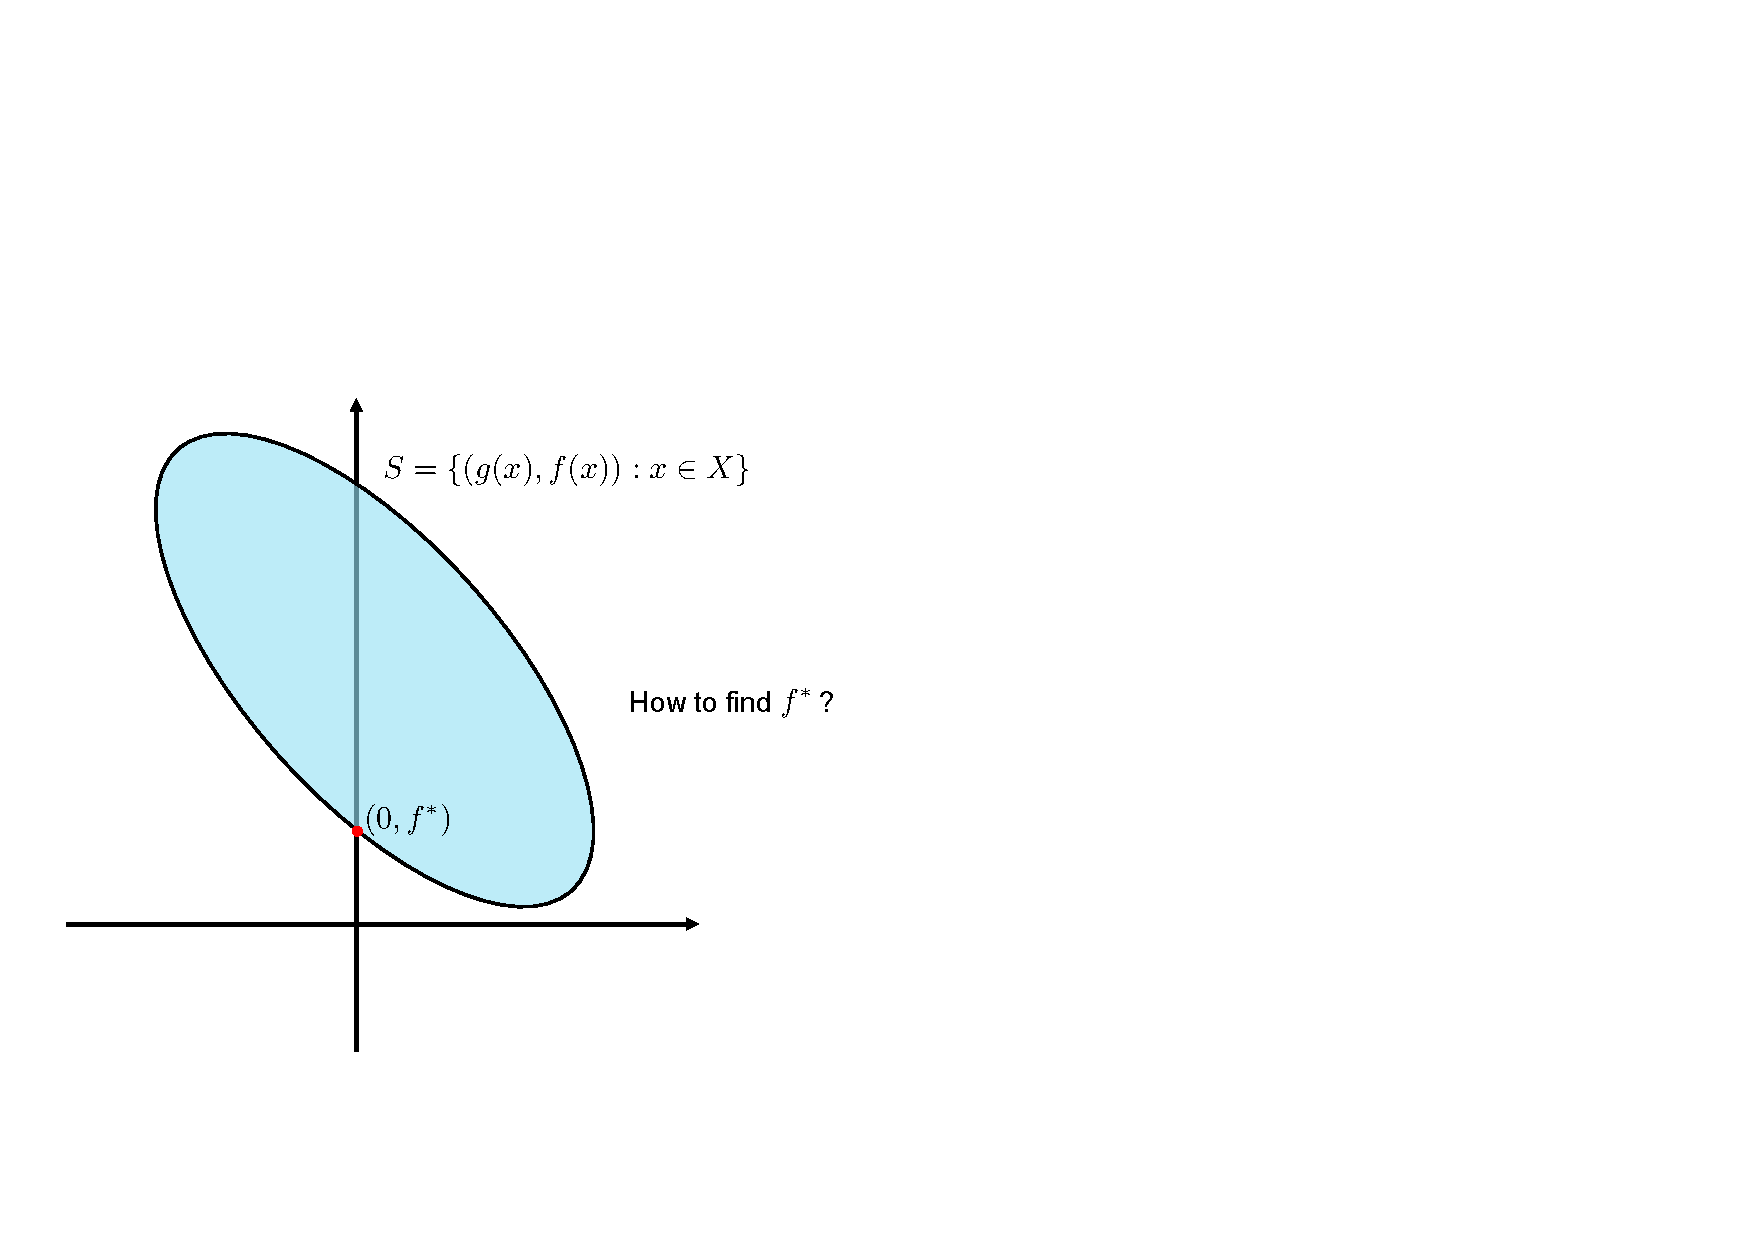
\includegraphics[width=0.45\columnwidth]{figures/geometric-multipliers-0.pdf}
		}
		\subfigure[] { \label{fig:geometric-multiplier-1}
			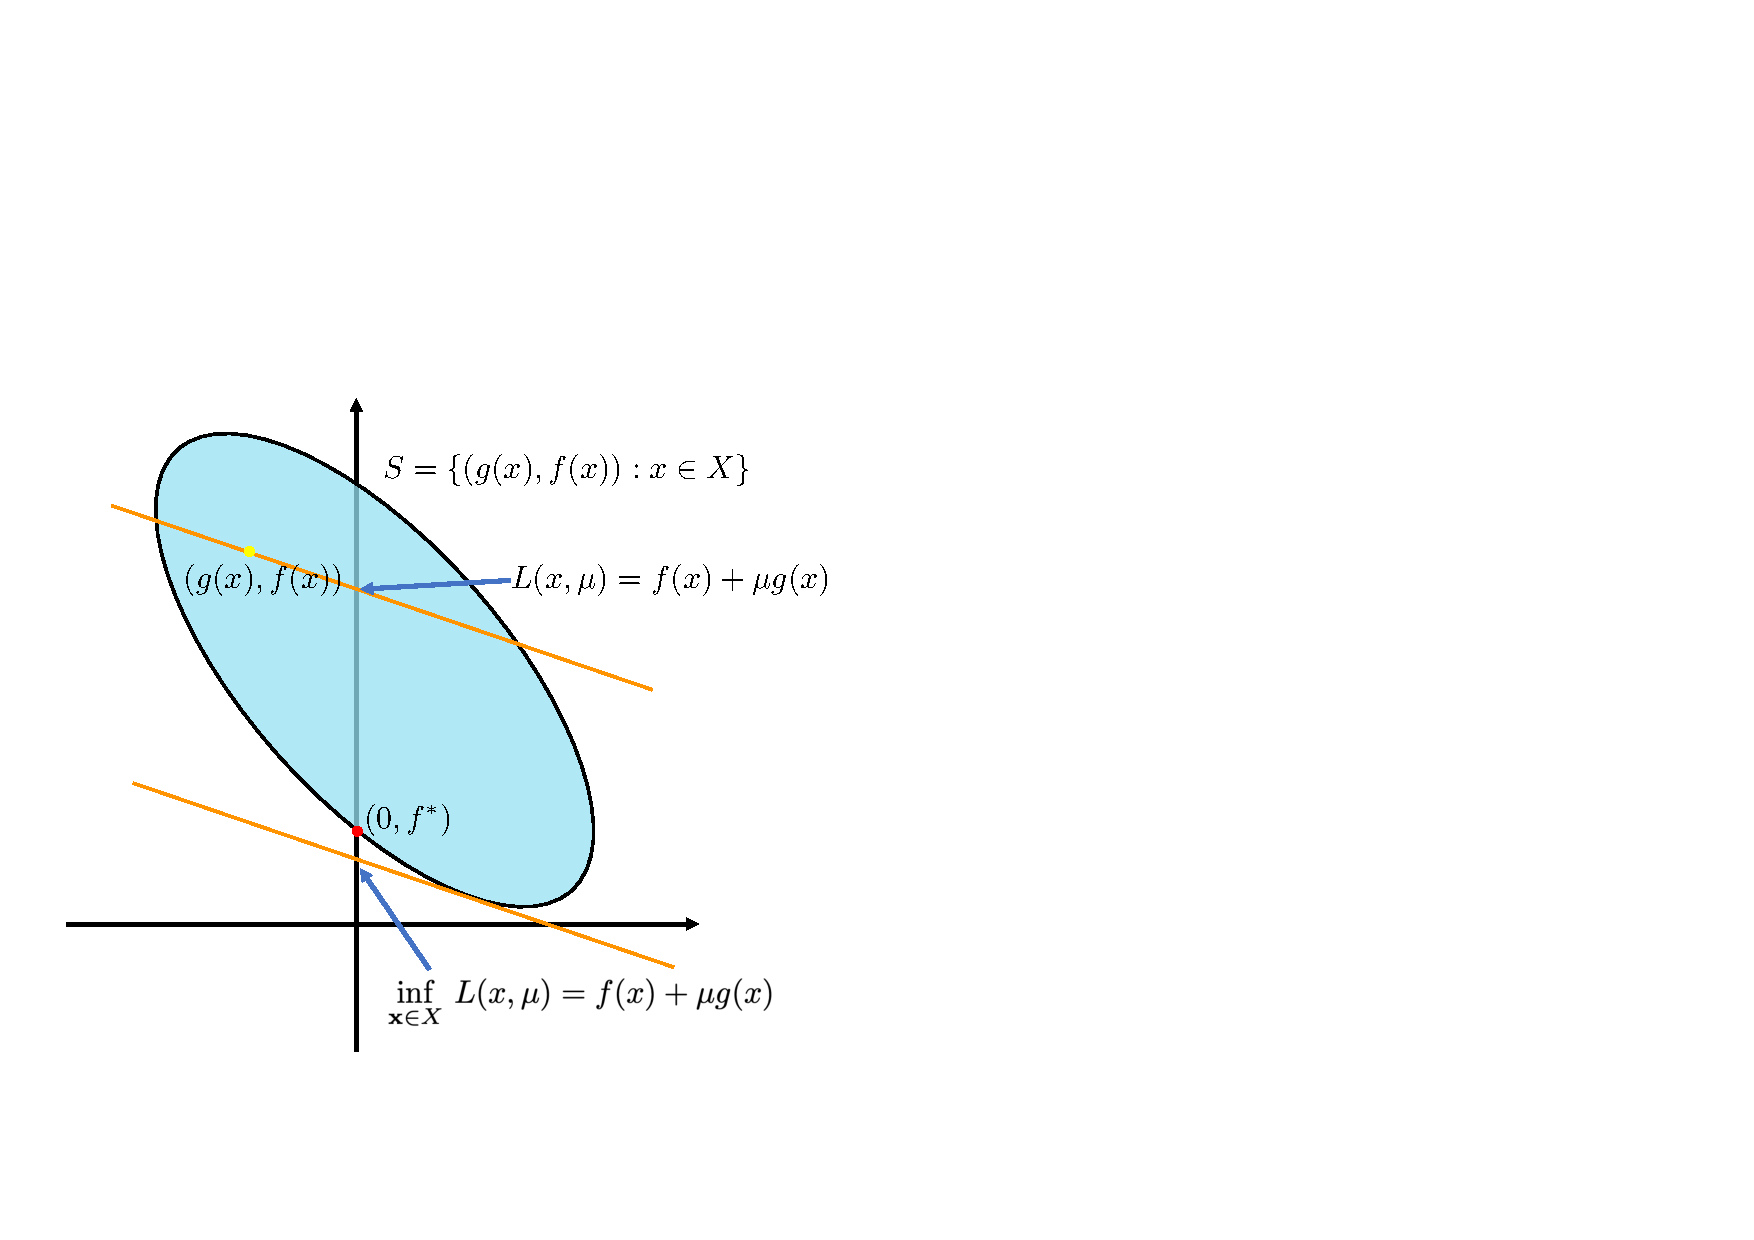
\includegraphics[width=0.45\columnwidth]{figures/geometric-multipliers-1.pdf}
		}
	}
	\caption{Illustration of the visualization lemma with one inequality constraint.}
	\label{fig:visualization-lemma}
\end{figure}



\newpage
${}$
\begin{solution}
	\heiti
	\begin{enumerate}
		\ \\
		\item 设空间的坐标为 $(\textbf{u}, \textbf{v}, w)$ ,其中 $\textbf{u} \in \mathbb{R}^m, \textbf{v} \in \mathbb{R}^p, w \in \mathbb{R}$,超平面的方程可以写为
		\begin{align*}
			F = \lambda \textbf{u} + \mu \textbf{v} + w
		\end{align*}
		因为超平面过 $(\mathbf{g}(\mathbf{x}),\mathbf{h}(\mathbf{x}),f(\mathbf{x}))$ ,则有:
		\begin{align*}
			\lambda \textbf{u} + \mu \textbf{v} + w = \lambda \mathbf{g}(\mathbf{x}) + \mu \mathbf{h}(\mathbf{x}) + f(\mathbf{x})
		\end{align*}
		可以看出当 $\textbf{u} = \textbf{v} = \textbf{0}$ 时,超平面交坐标轴于 $\lambda \mathbf{g}(\mathbf{x}) + \mu \mathbf{h}(\mathbf{x}) + f(\mathbf{x})$,此即为 $L(\mathbf{x},\lambda,\mu)$。
		\item 根据题目要求,超平面方程必须满足:
		\begin{align*}
			\lambda \textbf{u} + \mu \textbf{v} + w \leqslant \lambda \mathbf{g}(\mathbf{x}) + \mu \mathbf{h}(\mathbf{x}) + f(\mathbf{x})
		\end{align*}
		所以与坐标轴的交点满足:
		\begin{align*}
			w \leqslant \lambda \mathbf{g}(\mathbf{x}) + \mu \mathbf{h}(\mathbf{x}) + f(\mathbf{x})
		\end{align*}
		所能取到的最大值满足:
		\begin{align*}
			w = \inf_{\mathbf{x}\in X}\, \lambda \mathbf{g}(\mathbf{x}) + \mu \mathbf{h}(\mathbf{x}) + f(\mathbf{x}) = \inf_{\mathbf{x}\in X}\,L(\mathbf{x},\lambda,\mu)
		\end{align*}
		当超平面与 $S$ 有切点时取到等号。
		\item 根据定义如果 $\lambda^*, \mu^*$ 是 geometric multiplier,那么 $\lambda^* \geqslant 0, f^* = \inf L(\mathbf{x}, \lambda^*, \mu^*)$,所以超平面与纵轴的交点最高为 $\inf L(\mathbf{x}, \lambda^*,\mu^*) = f^*$。
		相反,如果满足 $\lambda^* \geqslant 0$,超平面与纵轴的交点最高为 $f^*$,这蕴含 $\inf L(\mathbf{x}, \lambda^*, \mu^*) = f^*$,根据 geometric multiplier 的定义,$(\lambda^*,\mu^*)$ 是 geometric multiplier。综上命题成立。
	\end{enumerate}
\end{solution}

\newpage
\begin{exercise}[Geometric Multiplier]
Let $(\lambda^*,\mu^*)$ be a geometric multiplier. Show that $\mathbf{x}^*$ is a global minimum of the primal problem (\ref{prob:primal-vec}) if and only if $\mathbf{x}^*$ is feasible and 
\begin{align*}
	&\mathbf{x}^*\in\argmin_{\mathbf{x}\in X}\,L(\mathbf{x},\lambda^*,\mu^*),\\
	&\lambda_i^*g_i(\mathbf{x}^*)=0,\,i=1,\ldots,m.
\end{align*}
\end{exercise}

\begin{solution}
	\heiti
	\ \\
	$\mathbf{x}^* \in X$ 说明 $\mathbf{g}(\mathbf{x^*}) \leqslant 0, \mathbf{h}(\mathbf{x^*}) = 0$,$\mathbf{x}^*$ 是问题 3 的最小值,则 $f^* = f(\mathbf{x}^*) = \min\{f(\mathbf{x}):\mathbf{g}(\mathbf{x})\leq0,\mathbf{h}(\mathbf{x})=0,\mathbf{x}\in X)\}$,根据 $(\lambda^*,\mu^*)$ 是 geometric multiplier 可得:
	\begin{align*}
		\min\{f(\mathbf{x}):\mathbf{g}(\mathbf{x})\leq0,\mathbf{h}(\mathbf{x})=0,\mathbf{x}\in X)\} = f^* = & \inf_{\mathbf{x}\in X}\,L(\mathbf{x},\lambda^*,\mu^*)\\
		= & \inf_{\mathbf{x}\in X}\,\{f(\mathbf{x})+\lambda^* \mathbf{g}(\mathbf{x})\}
	\end{align*}
	因为 $\lambda^* \geqslant 0$,所以 $\lambda^* \mathbf{g}(\mathbf{x}) \leqslant 0$,要使上式成立,那么 $\lambda^* \mathbf{g}(\mathbf{x}) = 0$,得:
	\begin{align*}
		L(\mathbf{x}^*,\lambda^*,\mu^*) = \min_{\mathbf{x}\in X}\,L(\mathbf{x},\lambda^*,\mu^*)
	\end{align*}
	所以 $\mathbf{x}^*\in\argmin_{\mathbf{x}\in X}\,L(\mathbf{x},\lambda^*,\mu^*)$ 并且 $\lambda^* \mathbf{g}(\mathbf{x}^*) = 0$。\\
	反之如果题中的条件成立,由于 $(\lambda^*,\mu^*)$ 是 geometric multiplier,所以 $\inf L(\mathbf{x}, \lambda^*, \mu^*) = f^*$,那么
	\begin{align*}
		L(\mathbf{x}^*,\lambda^*,\mu^*) = f(\mathbf{x}^*) + \lambda^*\mathbf{g}(\mathbf{x}^*) + \mu^*\mathbf{h}(\mathbf{x}^*) = f(\mathbf{x}^*)\\
		\Rightarrow f(\mathbf{x}^*) = L(\mathbf{x}^*,\lambda^*,\mu^*) = \min L(\mathbf{x},\lambda^*,\mu^*) = f^*
	\end{align*}
	所以 $\mathbf{x}^*$ 可以取到全局最小值,综上命题成立。
\end{solution}

\newpage
\begin{exercise}[Lagrange Dual Problem]
Consider the primal problem (\ref{prob:primal-vec}) and the Lagrangian (\ref{def:Lagrangian}). We define the dual function for $(\lambda,\mu)\in\mathbb{R}^{m+p}$ by
\begin{align*}
	q(\lambda,\mu)=\inf_{\mathbf{x}\in X}\,L(\mathbf{x},\lambda,\mu).
\end{align*}
The domain of $q$ is 
\begin{align*}
    \dom(q)=\{(\lambda,\mu):q(\lambda,\mu)>-\infty\}.
\end{align*}
The dual problem is
\begin{align*}
	\sup\,&q(\lambda,\mu),\\
	\mbox{s.t. }&\lambda\geq0.
\end{align*}
\begin{enumerate}
    \item Show that $\dom(q)$ is convex.
    \item Show that $-q(\lambda,\mu)$ is a convex function.
\end{enumerate}
\end{exercise}

\begin{solution}
	\heiti
	\ \\
	\begin{enumerate}
		\item 任取 $(\lambda_1, \mu_1), (\lambda_2, \mu_2) \in \dom(q)$,对于 $\forall \theta \in (0,1)$,考虑 $\theta(\lambda_1, \mu_1) + (1-\theta)(\lambda_2, \mu_2) = (\theta \lambda_1 + (1-\theta)\lambda_2, \theta \mu_1 + (1-\theta)\mu_2)$,有:
		\begin{align*}
			q(\theta \lambda_1 + (1-\theta)\lambda_2, \theta \mu_1 + (1-\theta)\mu_2) &=\inf_{\mathbf{x}\in X}\,L(\mathbf{x},\theta \lambda_1 + (1-\theta)\lambda_2, \theta \mu_1 + (1-\theta)\mu_2)\\
			&=\inf_{\mathbf{x}\in X}\,f(\mathbf{x})+(\theta \lambda_1 + (1-\theta)\lambda_2)g(\mathbf{x}) + (\theta \mu_1 + (1-\theta)\mu_2)h(\mathbf{x})\\
			&=\inf_{\mathbf{x}\in X}\,\theta L(\mathbf{x},\lambda_1, \mu_1) + (1-\theta)L(\mathbf{x}, \lambda_2, \mu_2)
		\end{align*}
		由于 $\inf_{\mathbf{x}\in X}\,L(\mathbf{x},\lambda_1,\mu_1) > -\infty, \inf_{\mathbf{x}\in X}\,L(\mathbf{x},\lambda_2,\mu_2) > -\infty$,故 $L(\mathbf{x},\lambda_1,\mu_1) > -\infty, L(\mathbf{x},\lambda_2,\mu_2) > -\infty$,所以 $\inf_{\mathbf{x}\in X}\,\theta L(\mathbf{x},\lambda_1, \mu_1) + (1-\theta)L(\mathbf{x}, \lambda_2, \mu_2) > -\infty$。由此可知 $\theta(\lambda_1, \mu_1) + (1-\theta)(\lambda_2, \mu_2) \in \dom(q)$,故是凸集。
		\item 任取 $(\lambda_1, \mu_1), (\lambda_2, \mu_2) \in \dom(q)$,对于 $\forall \theta \in (0,1)$,需要证明:
		\begin{align*}
			-q(\theta \lambda_1 + (1-\theta)\lambda_2, \theta \mu_1 + (1-\theta)\mu_2) &\leqslant -\theta q(\lambda_1,\mu_1) - (1-\theta)q(\lambda_2,\mu_2)\\
			\Leftrightarrow \inf_{\mathbf{x}\in X}\,\theta L(\mathbf{x},\lambda_1, \mu_1) + (1-\theta)L(\mathbf{x}, \lambda_2, \mu_2) &\geqslant \theta \inf_{\mathbf{x}\in X}\,  L(\mathbf{x},\lambda_1, \mu_1) + (1-\theta) \inf_{\mathbf{x}\in X}\, L(\mathbf{x}, \lambda_2, \mu_2)\\
		\end{align*}
		利用 $\theta \inf_{\mathbf{x}\in X}\,  L(\mathbf{x},\lambda_1, \mu_1) = \inf_{\mathbf{x}\in X}\, \theta L(\mathbf{x},\lambda_1, \mu_1), (1-\theta) \inf_{\mathbf{x}\in X}\, L(\mathbf{x}, \lambda_2, \mu_2) =  \inf_{\mathbf{x}\in X}\, (1-\theta) L(\mathbf{x}, \lambda_2, \mu_2)$,以及对于任意函数 $P,Q$ 有 $\inf(P+Q) \geqslant \inf P\,+ \inf Q$ 得:
		\begin{align*}
			\inf_{\mathbf{x}\in X}\,\theta L(\mathbf{x},\lambda_1, \mu_1) + (1-\theta)L(\mathbf{x}, \lambda_2, \mu_2) \geqslant  \inf_{\mathbf{x}\in X}\, \theta L(\mathbf{x},\lambda_1, \mu_1) +  \inf_{\mathbf{x}\in X}\,(1-\theta) L(\mathbf{x}, \lambda_2, \mu_2)
		\end{align*}
		成立,所以原命题成立。
	\end{enumerate}
\end{solution}



\newpage
\begin{exercise}[Duality Gap]
Duality gap is defined by
	\begin{align*}
		f^*-q^*.
	\end{align*}
	Show that the following results hold.
	\begin{enumerate}
		\item If there is no duality gap, the set of geometric multipliers is equal to the set of optimal dual solutions.
		\item If there is duality gap, the set of geometric multipliers is empty.
	\end{enumerate}
\end{exercise}

\begin{solution}
	\heiti
	\ \\
	\begin{enumerate}
		\item 由题,$f^* = q^*$,考虑 $q^*$:
		\begin{align*}
			q^* = \sup q(\lambda^*,\mu^*),\\
			s.t. \lambda^* \geq 0
		\end{align*}
		对于
		\begin{align*}
			q(\lambda,\mu) &= \inf_{\mathbf{x}\in X}\, L(\mathbf{x},\lambda,\mu)\\
			&= \inf_{\mathbf{x}\in X}\, \{f(\mathbf{x}) + \lambda \mathbf{g}(\mathbf{x}) + \mu \mathbf{h}(\mathbf{x})\}\\
			&\leqslant f(\mathbf{x}) + \lambda \mathbf{g}(\mathbf{x}) + \mu \mathbf{h}(\mathbf{x})
		\end{align*}
		对于 $\mathbf{x} \in X$,有 $\mathbf{h}(\mathbf{x}) = 0, \mathbf{g}(\mathbf{x}) \leqslant 0$,那么有 $\lambda\mathbf{g}(\mathbf{x}) \leqslant 0$,所以
		\begin{align*}
			q(\lambda,\mu) &\leqslant  f(\mathbf{x})\\
			\Rightarrow q^* =  \sup q(\lambda,\mu) &\leqslant \min f(\mathbf{x}) = f^*
		\end{align*}
		根据定义,如果 $(\lambda^*,\mu^*)$ 是 geometric multiplier,那么
		\begin{align*}
			q(\lambda^*,\mu^*) = f^*
		\end{align*}
		根据上面的推导
		\begin{align*}
			q(\lambda^*,\mu^*) \leqslant \sup q(\lambda,\mu) &= q^* \leqslant \min f(\mathbf{x})  \leqslant f^*\\
			\Rightarrow q(\lambda^*,\mu^*) &= q^* = f^*
		\end{align*}
		故综上,所有最优解 $(\lambda^*,\mu^*)$ 都满足 geometric multiplier 的定义,满足 geometric multiplier 定义的 $(\lambda^*,\mu^*)$ 同样是最优解,故命题成立。
		\item 假设 geometric multipliers 的集合不是空集,根据其定义
		\begin{align*}
			q(\lambda^*,\mu^*) = f^*
		\end{align*}
		由 1 的推导可推出 $q^* = q(\lambda^*,\mu^*) = f^*$,但这与 $f^* - q^* \neq 0$ 矛盾,故集合为空。
	\end{enumerate}
\end{solution}

\newpage
\begin{exercise}[Optimality Conditions]
	Show that a pair $\mathbf{x}^*$ and $(\lambda^*,\mu^*)$ is an optimal solution and geometric multiplier pair if and only if
	\begin{align}\label{cond:primal-feasibility}
		\mathbf{x}^*\in X,\,\mathbf{g}(\mathbf{x}^*)\leq0,\mathbf{h}(\mathbf{x}^*)=0,\hspace{18.5mm}(\mbox{\textup{Primal Feasibility}}),&\\ \label{cond:dual-feasibility}
		\lambda^*\geq0,\hspace{22mm}(\mbox{\textup{Dual Feasibility}}),&\\ \label{cond:lagrangian-optimality}
		\mathbf{x}^*\in\argmin_{\mathbf{x}\in X}\,L(\mathbf{x},\lambda^*,\mu^*),\hspace{10mm}(\mbox{\textup{Lagrangian Optimality}}),&\\ \label{cond:complementary-slackness}
		\lambda^*_ig_i(\mathbf{x}^*)=0,\,i=1,\ldots,m,\hspace{5mm}(\mbox{\textup{Complementary Slackness}}).&
	\end{align}
\end{exercise}

\begin{solution}
	\heiti
	\ \\
	如果 $\mathbf{x}^*, (\lambda^*,\mu^*)$ 是一对最优解和 geometric multiplier,那么首先要满足约束条件:
	\begin{align*}
		\mathbf{x}^*\in X,\,\mathbf{g}(\mathbf{x}^*)\leq0,\mathbf{h}(\mathbf{x}^*)=& 0\\
		\lambda^*\geq& 0
	\end{align*}
	根据 Exercise 3,还要满足
	\begin{align*}
		\mathbf{x}^*\in\argmin_{\mathbf{x}\in X}\,L(\mathbf{x},\lambda^*,\mu^*)\\
		\lambda^*_ig_i(\mathbf{x}^*)=0,\,i=1,\ldots,m
	\end{align*}
	相反,如果满足题目中的四个条件,那么有
	\begin{align*}
		f^* \leqslant f(\mathbf{x}^*) = L(\mathbf{x}^*,\lambda^*,\mu^*) \leqslant L(\mathbf{x},\lambda^*,\mu^*) = q(\lambda^*,\mu^*) \leqslant q^*
	\end{align*}
	由 Exercise 5 中 $q^* \leqslant f^*$ 可知等号成立,所以 $\mathbf{x}^*, (\lambda^*,\mu^*)$ 是一对最优解和 geometric multiplier。
\end{solution}

\newpage
\begin{exercise}[Saddle Point Interpretation]
	 Show that a pair $\mathbf{x}^*$ and $(\lambda^*,\mu^*)$ is an optimal solution-geometric multiplier pair if and only if $\mathbf{x}^*\in X$, $\lambda^*\geq0$, and $(\mathbf{x}^*,\lambda^*,\mu^*)$ is a saddle point of the Lagrangian, in the sense that
	\begin{align}\label{cond:saddle-Lagrangian}
		L(\mathbf{x}^*,\lambda,\mu)\leq L(\mathbf{x}^*,\lambda^*,\mu^*)\leq L(\mathbf{x},\lambda^*,\mu^*),\,\forall\,\mathbf{x}\in X,\,\lambda\geq0.
	\end{align}
\end{exercise}

\begin{solution}
	\heiti
	\ \\
	由 Exercise 6 知 $\mathbf{x}^*\in\argmin_{\mathbf{x}\in X}\,L(\mathbf{x},\lambda^*,\mu^*)$,故
	\begin{align*}
		L(\mathbf{x}^*,\lambda^*,\mu^*) \leqslant L(\mathbf{x},\lambda^*,\mu^*)
	\end{align*}
	由 Exercise 5 可得:
	\begin{align*}
		\sup q(\lambda,\mu) = q^* = q(\lambda^*,\mu^*)\\
		q(\lambda,\mu) = \inf_{\mathbf{x}\in X}\, L(\mathbf{x},\lambda,\mu) \leqslant \sup q(\lambda,\mu) = q(\lambda^*,\mu^*)
	\end{align*}
	因为 $x^*$ 是最优解,所以进一步有:
	\begin{align*}
		L(\mathbf{x}^*,\lambda,\mu) \leqslant L(\mathbf{x}^*,\lambda^*,\mu^*)
	\end{align*}
	相反,如果满足题中的不等式,右侧的不等式说明 $L(\mathbf{x}^*,\lambda^*,\mu^*) = \min{L(\mathbf{x},\lambda^*,\mu^*)}$,所以 $\mathbf{x}^* \in \argmin_{\mathbf{x}\in X}\,L(\mathbf{x}, \lambda^*,\mu^*)$。左侧的不等式说明 $\sup q(\lambda,\mu) = q^* = q(\lambda^*,\mu^*)$,即 $\lambda^*\mathbf{g}(\mathbf{x}^*) = 0$,综上并由 Exercise 6 知 $x^*, (\lambda^*, \mu^*)$ 是一对最优解和 geometric multiplier。\\
	故综上命题成立。
\end{solution}

\newpage
\begin{exercise}
     Recall that the soft margin SVM takes the form of
\begin{align}\label{prob:soft-SVM}
\min_{\mathbf{w},b,\xi}\,&\frac{1}{2}\|\mathbf{w}\|^2+C\sum_{i=1}^n\xi_i,\\ \nonumber
{\rm s.t.\,}&\,y_i(\langle\mathbf{w},\mathbf{x}_i\rangle+b)\geq1-\xi_i,i=1,\ldots,n,&\\ \nonumber
&\,\xi_i\geq0,\,i=1,\ldots,n,
\end{align}
where $C>0$.
The corresponding dual problem is
\begin{align}\label{prob:dual-soft-SVM}
		\min_{\alpha}\,&\frac{1}{2}\sum_{i=1}^n\sum_{j=1}^n\,\alpha_i\alpha_jy_iy_j\langle\mathbf{x}_i,\mathbf{x}_j\rangle-\sum_{i=1}^n\alpha_i\\\nonumber
	\mbox{s.t. }\,&\sum_{i=1}^n\alpha_iy_i=0,\\\nonumber
	&\alpha_i\in[0,C],i=1,\ldots,n.
\end{align}
\begin{enumerate}
    \item Show that the problems (\ref{prob:soft-SVM}) and (\ref{prob:dual-soft-SVM}) always admit optimal solutions.
    
    \item Suppose that the training data consists of two data instances $x_1=1$ and $x_2=-1$, and the corresponding labels are $y_1=1$ and $y_2=-1$.
    \begin{enumerate}
        \item Please solve problem (\ref{prob:SVM}) and find the primal and dual optimal solutions.
        \item Please solve problem (\ref{prob:soft-SVM}) with $C<\frac{1}{2}$ and find the primal and dual optimal solutions.
    \end{enumerate}

    \item Suppose that the training data consists of four data instances: $\mathbf{x}_1=(2,3)$, $\mathbf{x}_2=(1,2)$, $\mathbf{x}_3=(1,3)$, and $\mathbf{x}_4=(2,2)$, and the corresponding labels are $y_1=y_2=1$ and $y_3=y_4=-1$. Please solve the problem in (\ref{prob:dual-soft-SVM}) with $C=10$.
\end{enumerate}
Notice that, for the last two parts, you need to find all the primal and dual optimal solutions if they are not unique.
\end{exercise}

\begin{solution}
	\heiti
	\ \\
	\begin{enumerate}
		\item 对于问题 11,不妨取 $\mathbf{w} = \mathbf{0}, b = 0$,那么有:
		\begin{align*}
			0 &\geqslant 1 - \xi_i\\
			\Rightarrow \xi_i &\geqslant 1
		\end{align*}
		可以取 $\xi_i = 2$,于是得到一组解(必定有解),此时目标函数的值为 $2nC$。目标函数要取到最小值,那么 $\mathbf{w}, \xi_i$,必为有限值,故只能在闭集内取到最小值,解集非空,所以一定有最优解。\\
		对于问题 12,容易看出 $\alpha_i = 0, i= 1,\dots, n$ 就是满足约束条件的一组 $\alpha$,所以解必定存在。当 $\alpha_i \rightarrow \infty$ 时,目标函数也趋于无穷,故一定在有限区间上取到最优解,解集非空,所以一定有最优解。
		\item \ \\
		\begin{enumerate}
			\item 根据约束条件有:
			\begin{align*}
				1(w+b) \geqslant 1\\
				-1(-w + b) \geqslant 1\\
				\Rightarrow w \geqslant 1 + b
			\end{align*}
			所以 $b = 0$ 时,$w = 1$ 取到最小值,这时目标函数最小值为 $\frac{1}{2}$。\\
			对偶问题可以写为
			\begin{align*}
				\max_{\alpha} &\sum\limits_{i=1}^{2} \alpha_i - \frac{1}{2}(\alpha_1^2y_1^2\langle x_1, x_1 \rangle + \alpha_2^2y_2^2\langle x_2, x_2 \rangle +2\alpha_1\alpha_2y_1y_2\langle x_1, x_2 \rangle)\\
				&= \alpha_1 + \alpha_2 - \frac{1}{2}(\alpha_1^2 + \alpha_2^2 + 2\alpha_1\alpha_2)\\
				&= \alpha_1 + \alpha_2 - \frac{1}{2} (\alpha_1 + \alpha_2)^2\\
				&s.t. \alpha_1-\alpha_2 = 0,\\
				&\alpha_i \geqslant 0, i= 1, 2
			\end{align*}
			代入下面的条件得:
			\begin{align*}
				\max_{\alpha} 2\alpha_1(1-\alpha_1)
			\end{align*}
			所以 $\alpha_1 = \alpha_2 = \frac{1}{2}$ 是对偶问题的解,进一步可得 $w = 1, b = 0$。
			\item 根据约束条件有:
			\begin{align*}
				w + b \geqslant 1 - \xi_1\\
				w - b \geqslant 1 - \xi_2\\
				\Rightarrow w \geqslant 1 - \frac{\xi_1}{2} - \frac{\xi_2}{2}
			\end{align*}
			代入目标函数得:
			\begin{align*}
				\frac{1}{2}\| 1-\frac{\xi_1}{2}-\frac{\xi_2}{2} \|^2 +C\xi_1 + C\xi_2
			\end{align*}
			函数分别对$\xi_1, \xi_2$求偏导数并令其等于 0,可得:
			\begin{align*}
				\frac{\xi_1}{4} + \frac{\xi_2}{4} = \frac{ 1 }{ 2} - C
			\end{align*}
			代入上面的式子可得:
			\begin{align*}
				w \geqslant 2C
			\end{align*}
			故 $w = 2C, \xi_1 + \xi_2 = 2-4C$ 时,函数取到最小值 $2C(1-C)$。\\
			对于对偶问题,同上一题类似可以得到
			\begin{align*}
				\min_{\alpha} 2\alpha_1(\alpha_1 - 1)
			\end{align*}
			根据 $\alpha_i \in [0, C]$ 可得,$\alpha_1 = \alpha_2 = C$ 是对偶问题的解。
		\end{enumerate}
		\item 使用二次规划的方法求解,将问题转化为如下形式
		\begin{align*}
			\min_{\alpha} &\frac{1}{2} \alpha^{\top}\mathbf{P}\alpha + \mathbf{q}^{\top}\alpha,\\
			s.t. &\sum\limits_{i=1}^n \alpha_iy_i = 0,\\
			&-\alpha_i \leqslant 0, i= 1,\dots, n,\\
			&\alpha_i \leqslant 10, i= 1,\dots, n.
		\end{align*}
		其中 $\mathbf{P}_{ij} = y_iy_j\langle\mathbf{x}_i,\mathbf{x}_j\rangle, \mathbf{q}^{\top} = (-1, -1, -1, -1)$,约束条件也写成矩阵形式可得:
		\begin{align*}
			\min_{\alpha} &\frac{1}{2} \alpha^{\top}\mathbf{P}\alpha + \mathbf{q}^{\top}\alpha,\\
			s.t. &\mathbf{G}\alpha \leqslant \mathbf{h}\\
			&\mathbf{A}\alpha = \mathbf{b}
		\end{align*}
		用 Python 调用 cvxopt 求解此问题得 $\alpha = (10, 10, 10, 10)$(程序代码见 solve.py)。
	\end{enumerate}
\end{solution}

%%%%%%%%%%%%%%%%%%%%%%%%%%%%%%%%%%%%%%%%%%%%%%%%%%%%%%%%%%%%%%%%

\end{document}
